% Caption for figures/fig_reliability_top{10,15,20,30,50}.{pdf,png}
% Split: short figure caption (main text) + full detail in Appendix (suppsec:synth_data).

% ============================ MAIN TEXT: figure ============================
\begin{figure}[h]
  \centering
  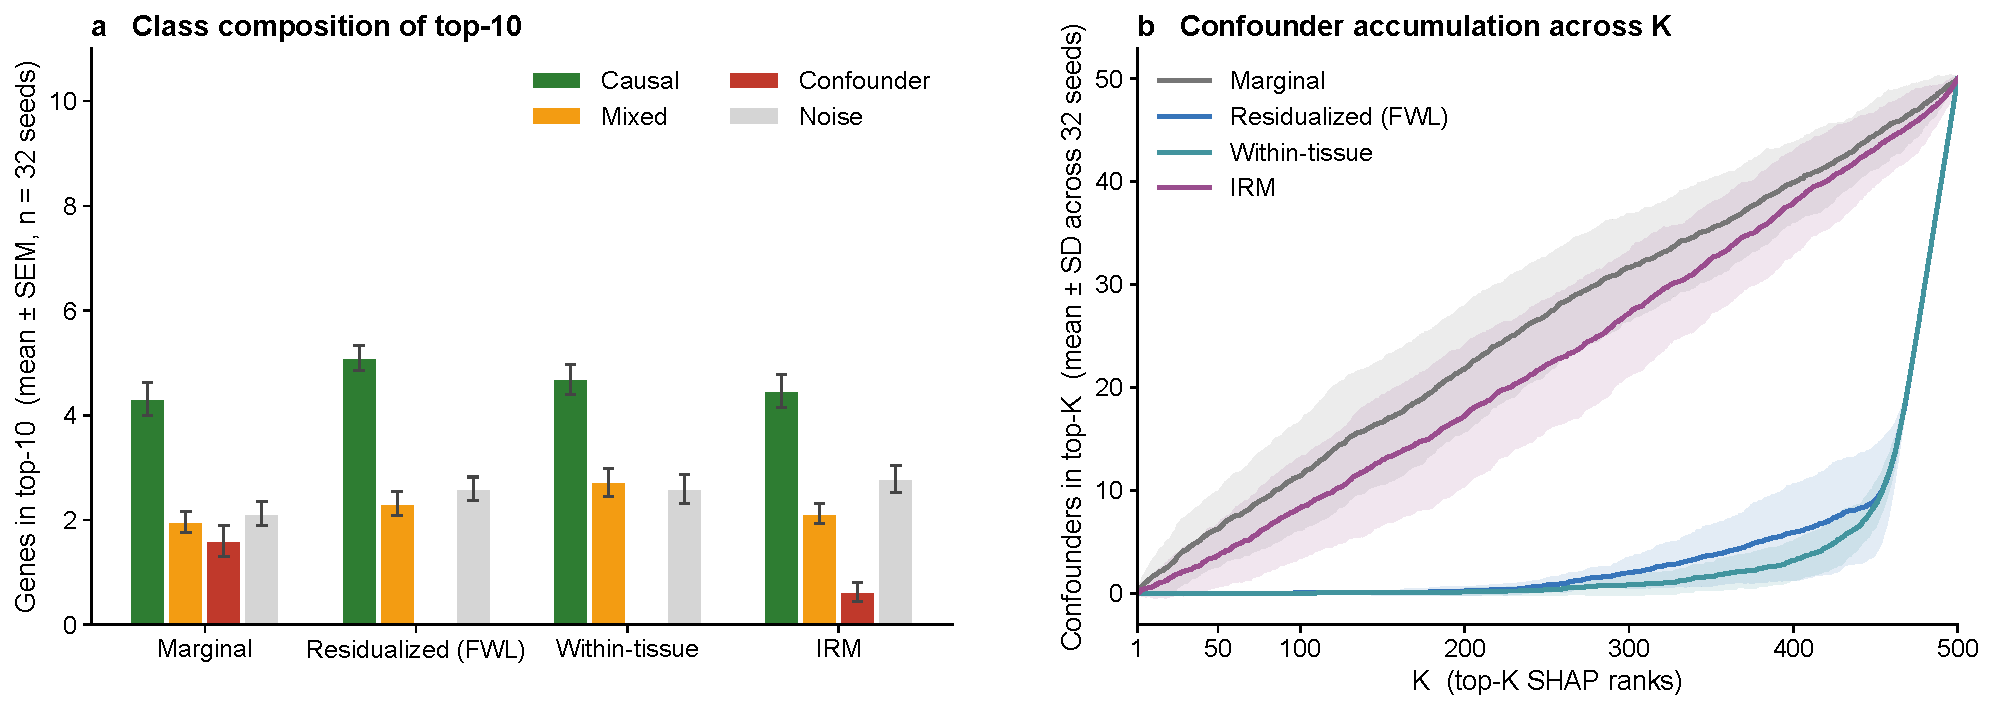
\includegraphics[width=\linewidth]{figures/fig_reliability_top10.pdf}
  \caption{\textbf{Synthetic experiments with known ground-truth confounder and causal genes.}
    The four explanation methods are run on $32$ independent replicates of a synthetic sample of $n=1000$ cells, $P=500$ genes across $T=12$ tissues, in which each gene is one of four \emph{known} classes: causal ($200$; affect the response $y$), mixed ($100$; causal \emph{and} tissue-amplified), confounder ($50$; pure tissue markers with no effect on $y$), and noise ($150$; inert). The data-generating process and the training and attribution setup are in Appendix~\ref{suppsec:synth_data}.
%
    \textbf{a}, Class composition of the top-10 important genes as determined by the methods, depicted as mean count of the classes (causal, mixed, confounder, noise) among the top-10 SHAP-ranked genes, averaged over the 32 seeds with standard error. Residualized and within-tissue Shapley return exactly zero confounders in the top-10 on every seed, and instead place more causal and mixed genes there than marginal, so deconfounding costs no true signal.
%
    \textbf{b}, Cumulative confounder count in the top-$K$ for $K=1,\dots,500$, one curve per method; shaded bands are the standard deviation across seeds. Residualized and within-tissue Shapley demote all confounders to the floor of the ranking.
  }
  \label{suppfig:synth_data}
\end{figure}

% ===================== APPENDIX: full experimental detail =====================
% Place in the supplementary section; this block carries \label{suppsec:synth_data}.
\subsection{Synthetic ground-truth data and attribution setup}
\label{suppsec:synth_data}

Each of the $32$ replicates draws an independent synthetic sample of $n=1000$ cells from a panel of $P=500$ genes across $T=12$ tissues (with unequal tissue sizes: Gamma$(2,1)$ weights normalized to the sample). Every gene belongs to one of four classes: \emph{causal} ($200$; affect the response $y$ and has ordinary tissue structure), \emph{mixed} ($100$; causal but also tissue-amplified in expression), \emph{confounder} ($50$ pure tissue markers with no effect on $y$: $15$ strongly amplified, $35$ weakly), and \emph{noise} ($150$). Expression is $X_{cg}=\mu_{t(c)g}+\varepsilon_{cg}$ with a tissue-specific mean $\mu_{tg}\sim\mathcal{N}(0,1)$ and within-tissue noise $\varepsilon\sim\mathcal{N}(0,1)$, plus additional tissue amplification for the mixed (amplitude $\mathrm{SD}=1$) and confounder genes (strong: $\mathrm{SD}=9$, noise $0.1$; weak: $\mathrm{SD}=6$, noise $1$). The response is $y_c = y^{\text{tissue}}_{t(c)} + \tanh\!\big(X_c[\text{causal+mixed}]\,\beta\big) + \eta_c$ with $\eta\sim\mathcal{N}(0,2^2)$; the between-tissue baseline $y^{\text{tissue}}$ is a random projection of the confounders' tissue signature (coupling $1.0$), so confounders predict $y$ purely through tissue identity at the population level while mixed genes have a causal signal that is also tissue-amplified. The per-gene causal coefficients are from classes strong/medium/weak/very-weak (fractions $0.05/0.15/0.30/0.50$ of the $300$ causal$+$mixed genes; magnitudes $4.0/1.6/0.6/0.12\times$ scale $0.085$, random sign).

All four methods use the same sample, an $85/15$ train/validation split, and standardized inputs. The predictor is a $2$-hidden-layer MLP ($128\!\to\!64$, ReLU, dropout $0.3$; Adam, learning rate $10^{-3}$, weight decay $10^{-4}$, batch $64$, up to $70$ epochs with early stopping). Results are in~\Cref{suppfig:synth_data}.
